\documentclass[letterpaper]{article}

\usepackage{amsmath}
\usepackage{amssymb}
\usepackage{amsthm}
\usepackage{commath}
\usepackage{enumerate}
\usepackage{lmodern}
\usepackage{microtype}
\usepackage{fullpage}
\usepackage{graphicx}

\title{STAT 527: Assignment \#2}
\author{Philip Pham}
\date{\today}

\DeclareMathOperator{\E}{E}
\DeclareMathOperator{\Prob}{P}

\begin{document}
\maketitle

\section*{Problem 1}

\begin{enumerate}[(a)]
\item
  \begin{proof}
    The likelihood function is the probability of observing the data.
    \begin{align*}
      L\left(\{y_{i,n}\}; f,\sigma\right)
      &= \prod_{i=1}^n \Prob\left(y_{i,n}; f, \sigma\right) \\
      &= \prod_{i=1}^n \frac{1}{\sqrt{2\pi\sigma^2}}\exp\left(
        -\frac{1}{2}\left(\frac{y_{i,n} - f\left(i/n\right)}{\sigma}\right)^2\right)
    \end{align*}
  \end{proof}
\item The approach is reasonable especially if we choose $f$ such that the
  likelihood is a differentiable function of the parameters. Then, it is easy to
  choose the optimal $\hat{f}$.
  
  Such an approach may be undesirable if our family of functions is too simple
  (high bias) or is not expressive enough (high variance). There may be other
  issues like the number of parameters that can lead to overfitting.
\item We can maximize the log-likelihood:
  \begin{align*}
    l\left(\{y_{i,n}\}; \mu,\sigma\right)
    &= -\frac{n}{2}\log\left(2\pi\sigma^2\right)  - \frac{1}{2\sigma^2}\sum_{i=1}^n\left(y_{i,n} - \mu\right)^2.
  \end{align*}
  Taking the derivative with respect to $\mu$ and solving, we get
  $\hat{\mu} = n^{-1}\sum_{i=1}^n y_{i,n}$, that is, the mean of observations.

  For the localization, we take a local mean:
  \begin{align*}
    f(x_0)
    &=
      \frac{\sum_{i=1}^n K_h\left(1/n - x_0\right)y_{i,n}}{\sum_{i=1}^n K_h\left(1/n - x_0\right)}, \\
    K_h\left(x\right) &= \begin{cases}
      1, &|x| \leq h; \\
      0, &\text{otherwise.}
    \end{cases}
  \end{align*}
  This is just the Nadaraya-Watson estimator with a box kernel with bandwidth
  $h$.
\end{enumerate}
\section*{Problem 2}
\begin{proof}
  Note that
  \begin{align*}
    \hat{\mu}_n
    &= \frac{1}{n}\sum_{i \leq n}x_i \sim \mathcal{N}\left(\mu, \frac{\sigma^2}{n}\right) \\
    n\frac{\hat{\sigma}^2_n}{\sigma^2} \sim \chi^2_{n-1}
    &\Rightarrow
      \hat{\sigma}^2_n
      = \frac{1}{n}\sum_{i \leq n}\left(x_i - \hat{\mu}\right)^2
      \sim \frac{\sigma^2}{n}\chi^2_{n-1}.
  \end{align*}
  Thus, we have $\E\left[\hat{\sigma}^2_n\right] = \frac{n-1}{n}\sigma^2$ and
  $\operatorname{var}\left(\hat{\sigma}^2_n\right) = 2\frac{n-1}{n^2} = 2/n -
  2/n^2$. Thus, the estimators are consistent. Using independence, Slusky's
  threom, and central limit theorem, we'll have have that
  \begin{equation*}
    \sqrt{n}\left(\begin{pmatrix}
      \hat{\mu}_n \\
      \hat{\sigma}_n
    \end{pmatrix} - \begin{pmatrix}
      \mu \\
      \sigma
    \end{pmatrix}\right)
  \xrightarrow{D}
  \mathcal{N}\left(
    \mathbf{0},
    \begin{pmatrix}
      \sigma^2 & 0 \\
      0 & 2
    \end{pmatrix}
  \right).
\end{equation*}

The delta method tells us that
  \begin{equation*}
    \sqrt{n}\left(
      \phi_{\hat{\mu},\hat{\sigma}}(x_0) - \phi_{\mu,\sigma}(x_0)
    \right)
  \xrightarrow{D}
  \mathcal{N}\left(
    \mathbf{0},
    \nabla\phi_{\mu,\sigma}(x_0)^\top
    \begin{pmatrix}
      \sigma^2 & 0 \\
      0 & 2
    \end{pmatrix}
    \nabla\phi_{\mu,\sigma}(x_0)
  \right),
\end{equation*}
where the gradient is evaluated with respect to $\mu$ and $\sigma$.

This just multiplies the diagonals by some constants and doesn't change the rate
of convergence. Convergence in distribution implies stochastic boundness, so
squaring both sides we have that
\begin{equation*}
  \left(\phi_{\hat{\mu},\hat{\sigma}}(x_0) - \phi_{\mu,\sigma}(x_0)\right)^2
  = O_p\left(1/n\right).
\end{equation*}
\end{proof}

\section*{Problem 3}
\begin{enumerate}[(a)]
\item See Figures \ref{fig:2fold}, \ref{fig:5fold}, and \ref{fig:10fold}
  \begin{figure}
    \caption{2-fold cross validation}
    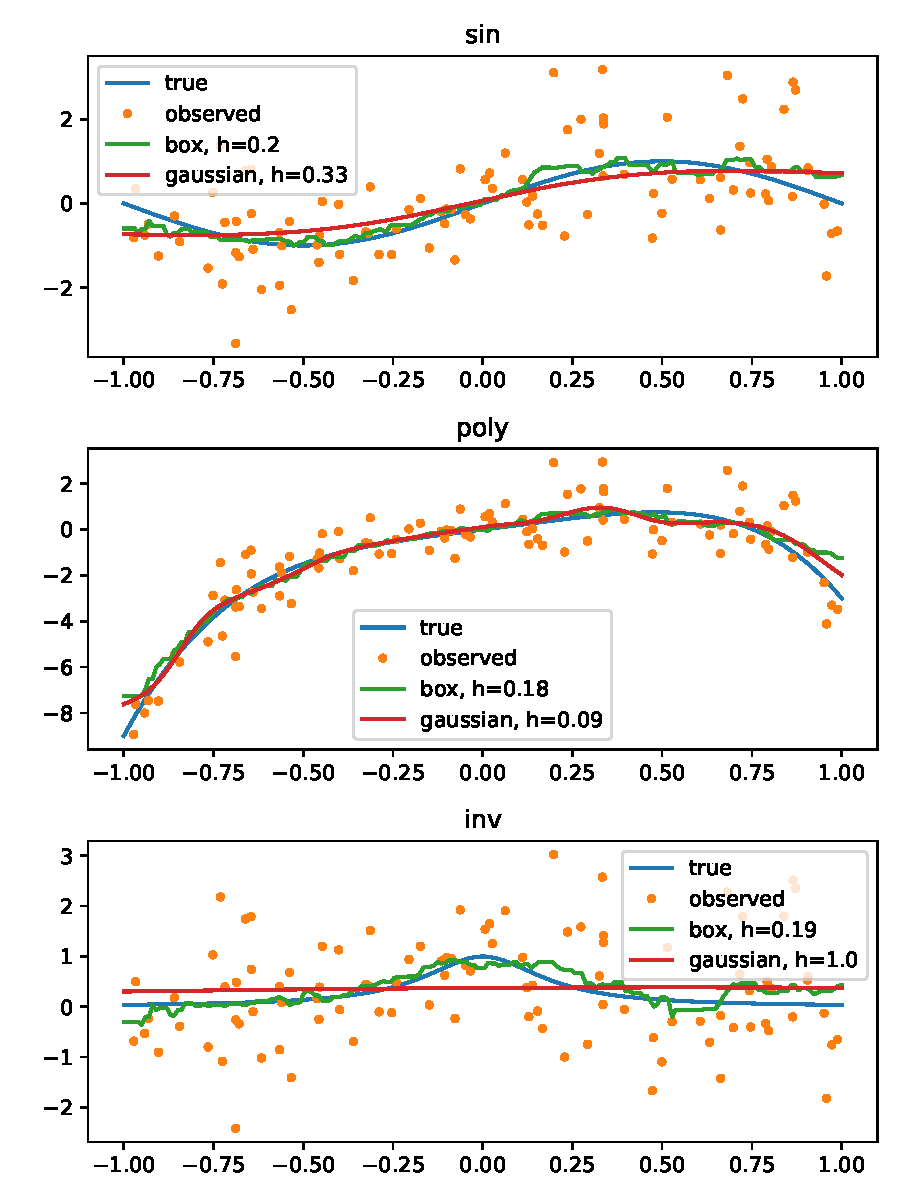
\includegraphics{cv_kernel_regression_2.pdf}
    \label{fig:2fold}
  \end{figure}

  \begin{figure}
    \caption{5-fold cross validation}
    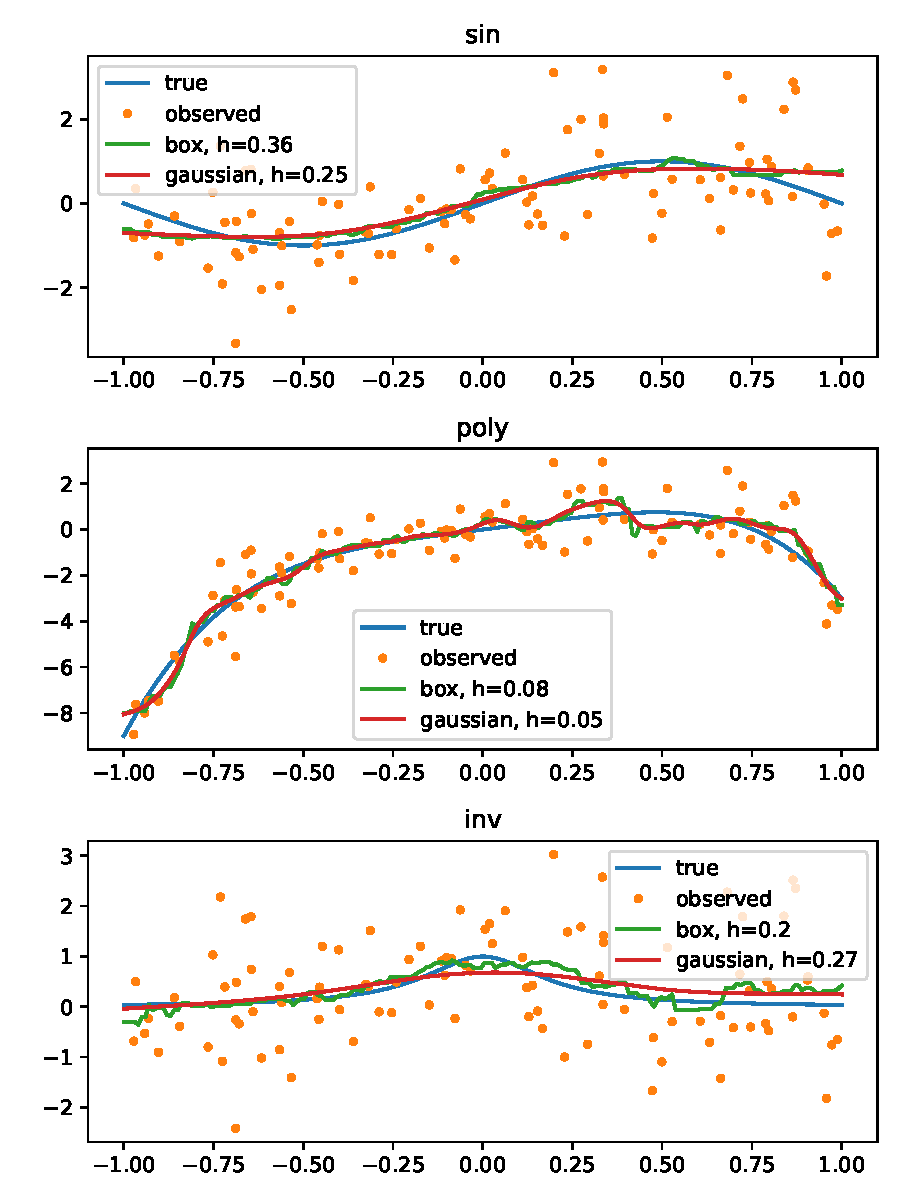
\includegraphics{cv_kernel_regression_5.pdf}
    \label{fig:5fold}
  \end{figure}

  \begin{figure}
    \caption{10-fold cross validation}
    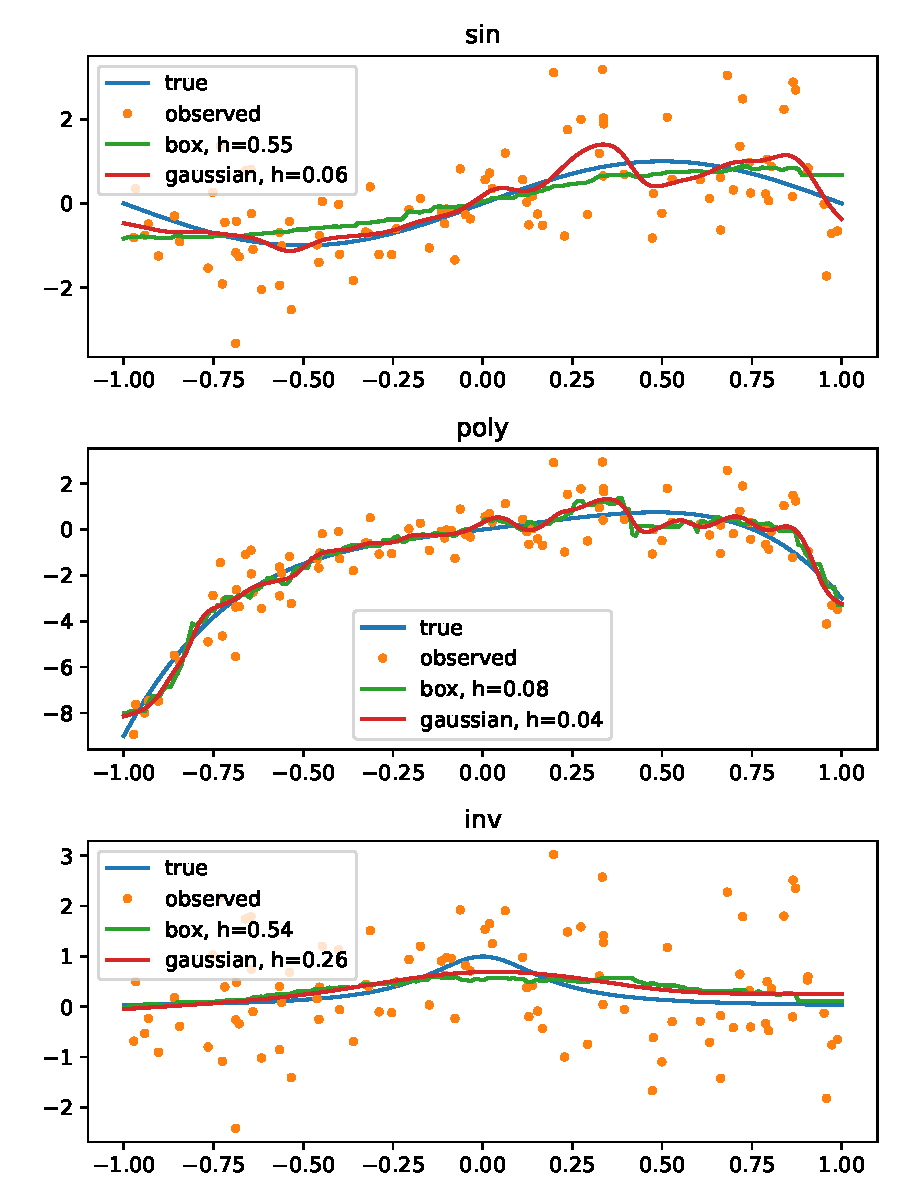
\includegraphics{cv_kernel_regression_10.pdf}
    \label{fig:10fold}
  \end{figure}

  While the trend isn't perfect, in general the larger $k$ tend to choose
  smaller bandwidths and more closely fit the data or sometimes noise.
\item After running 100 random folds, the following bandwidths were found.
  {\footnotesize
  \begin{verbatim}
[Summary(f='sin', kernel='box', oracle=0.25, k=2, mean=0.42499999999999993, var=0.025345),
 Summary(f='sin', kernel='box', oracle=0.25, k=5, mean=0.41139999999999993, var=0.03555404),
 Summary(f='sin', kernel='box', oracle=0.25, k=10, mean=0.39749999999999985, var=0.040248750000000014),
 Summary(f='sin', kernel='gaussian', oracle=0.13, k=2, mean=0.20759999999999998, var=0.01192024),
 Summary(f='sin', kernel='gaussian', oracle=0.13, k=5, mean=0.14210000000000003, var=0.0072085900000000026),
 Summary(f='sin', kernel='gaussian', oracle=0.13, k=10, mean=0.12510000000000002, var=0.006662989999999999),
 Summary(f='poly', kernel='box', oracle=0.11, k=2, mean=0.11530000000000001, var=0.0013089100000000008),
 Summary(f='poly', kernel='box', oracle=0.11, k=5, mean=0.08289999999999997, var=0.00011058999999999996),
 Summary(f='poly', kernel='box', oracle=0.11, k=10, mean=0.08079999999999998, var=1.535999999999999e-05),
 Summary(f='poly', kernel='gaussian', oracle=0.08, k=2, mean=0.061200000000000004, var=0.00032255999999999984),
 Summary(f='poly', kernel='gaussian', oracle=0.08, k=5, mean=0.049699999999999994, var=6.491000000000001e-05),
 Summary(f='poly', kernel='gaussian', oracle=0.08, k=10, mean=0.04869999999999999, var=1.731000000000001e-05),
 Summary(f='inv', kernel='box', oracle=0.33, k=2, mean=0.4341, var=0.03649419),
 Summary(f='inv', kernel='box', oracle=0.33, k=5, mean=0.36940000000000006, var=0.028043640000000015),
 Summary(f='inv', kernel='box', oracle=0.33, k=10, mean=0.42399999999999993, var=0.024012000000000002),
 Summary(f='inv', kernel='gaussian', oracle=0.2, k=2, mean=0.3048, var=0.06769296),
 Summary(f='inv', kernel='gaussian', oracle=0.2, k=5, mean=0.2088, var=0.014752560000000001),
 Summary(f='inv', kernel='gaussian', oracle=0.2, k=10, mean=0.1886, var=0.008036040000000001)]
\end{verbatim}}
    
    In general, bigger $k$ chose smaller bandwidths with less variance. There
    are some exceptions like with $k = 10$ and
    $f(x) = \left(1 + 25x^2\right)^{-1}.$ This tendency to choose a smaller
    bandwidth can sometimes lead to overfitting as it chooses a bandwidth
    smaller than the the oracle.
\end{enumerate}
\end{document}
